\documentclass[aspectratio=169]{beamer}
\usetheme{metropolis}

\usepackage[english]{babel}

\usepackage[scale=2]{ccicons}
\usepackage[framemethod=tikz]{mdframed}

\usepackage{graphicx}

\definecolor{titleframecolor}{HTML}{23373B}
\definecolor{titlebackgroundcolor}{HTML}{FAFAFA}

%Information to be included in the title page:
\title{The Age of Surveillance Capitalism}
\subtitle{Crypto Party Tirana}
\author{Ritger Teunissen (ritger@hack42.nl)}
\institute{OpenLabs (Tirana) \& Hack42 (Arnhem)}
\date{\today}

\setbeamertemplate{frame footer}{Crypto Party (\today)}
%\setbeameroption{show notes}
%\setbeameroption{show notes on second screen}

\newmdenv[tikzsetting={draw=titleframecolor,fill=titlebackgroundcolor,fill opacity=0.8, line width=1pt},
      backgroundcolor=none,leftmargin=0,rightmargin=0,innertopmargin=7pt]
      {titlebox}

\begin{document}
    \maketitle

    \begin{frame}{Table of Contents}
        \setbeamertemplate{section in toc}[sections numbered]
        \tableofcontents[hideallsubsections]
    \end{frame}

    {%
    \usebackgroundtemplate{\tikz\node[opacity=0.3,inner sep=0] {
\includegraphics[height=\paperheight]{images/milosz-klinowski-unsplash.jpg}};}
    \begin{frame}{\$ whoami}
        \begin{itemize}
            \item Husband, dad, nerd
            \item Worked in IT security for the last 13 years
            \item Member of hackerspace Hack42, Arnhem, The Netherlands
        \end{itemize}
    \end{frame}
    }

    \section{Discovery of Behavioural Surplus}%
    \label{sec:discovery_of_behavioural_surplus}

    {%
    \usebackgroundtemplate{\tikz\node[opacity=0.3,inner sep=0] {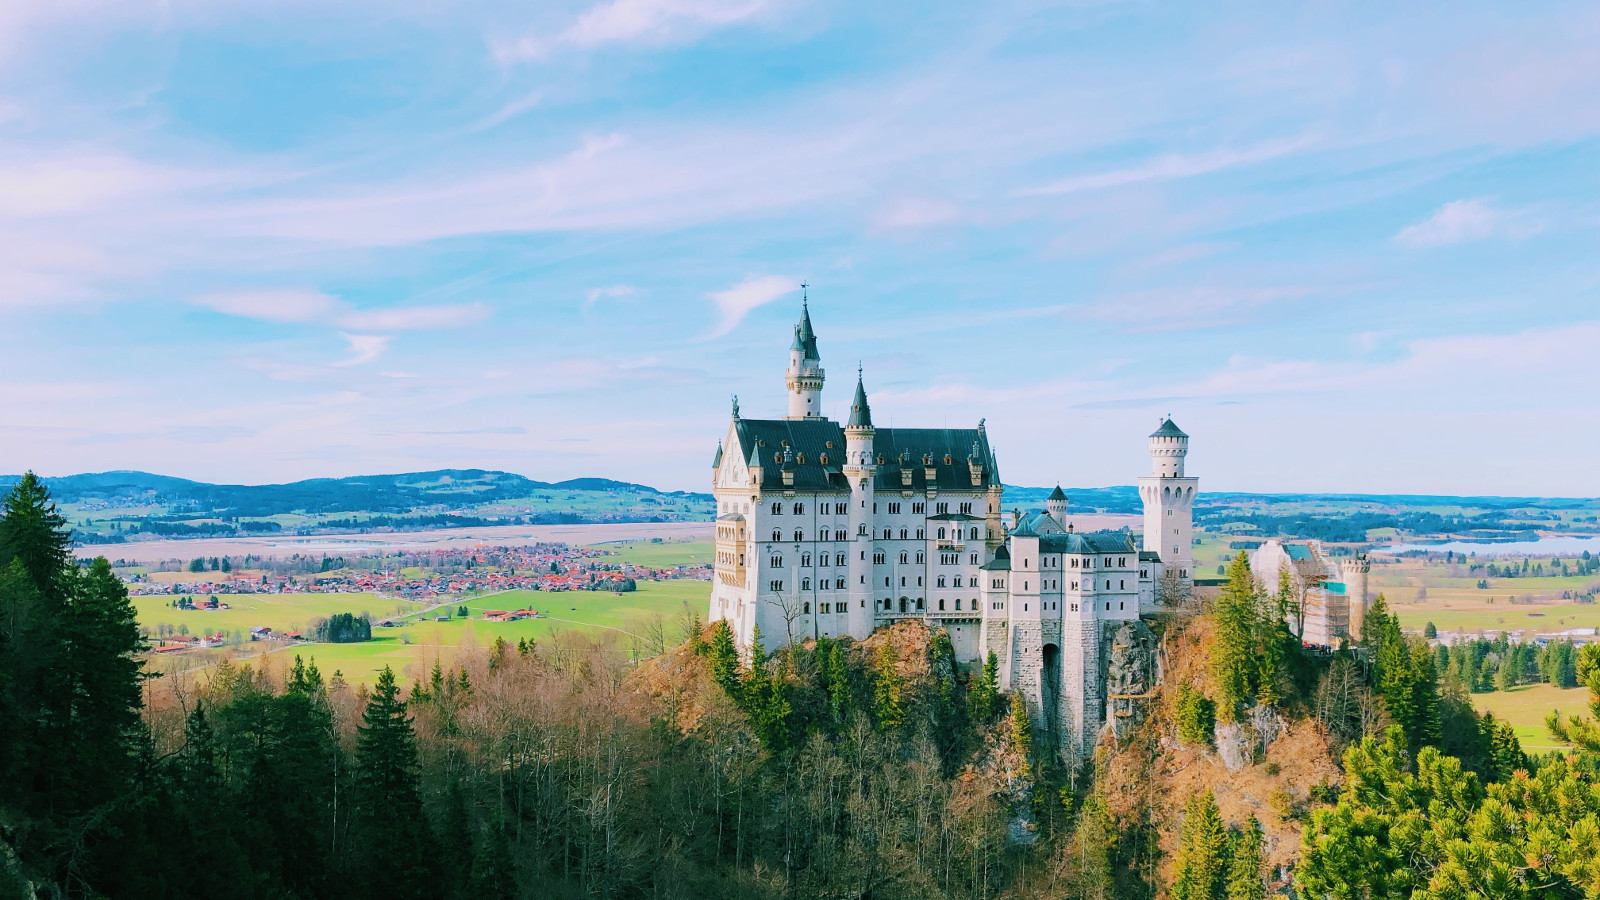
\includegraphics[height=\paperheight]{images/alex-vasey-unsplash.jpg}};}
    \begin{frame}{Once Upon a Time \ldots{}}
        \begin{itemize}
            \item There was a small company that built a search engine
            \item You may have heard of them \ldots{}
        \end{itemize}
    \end{frame}
    }

    {%
    \usebackgroundtemplate{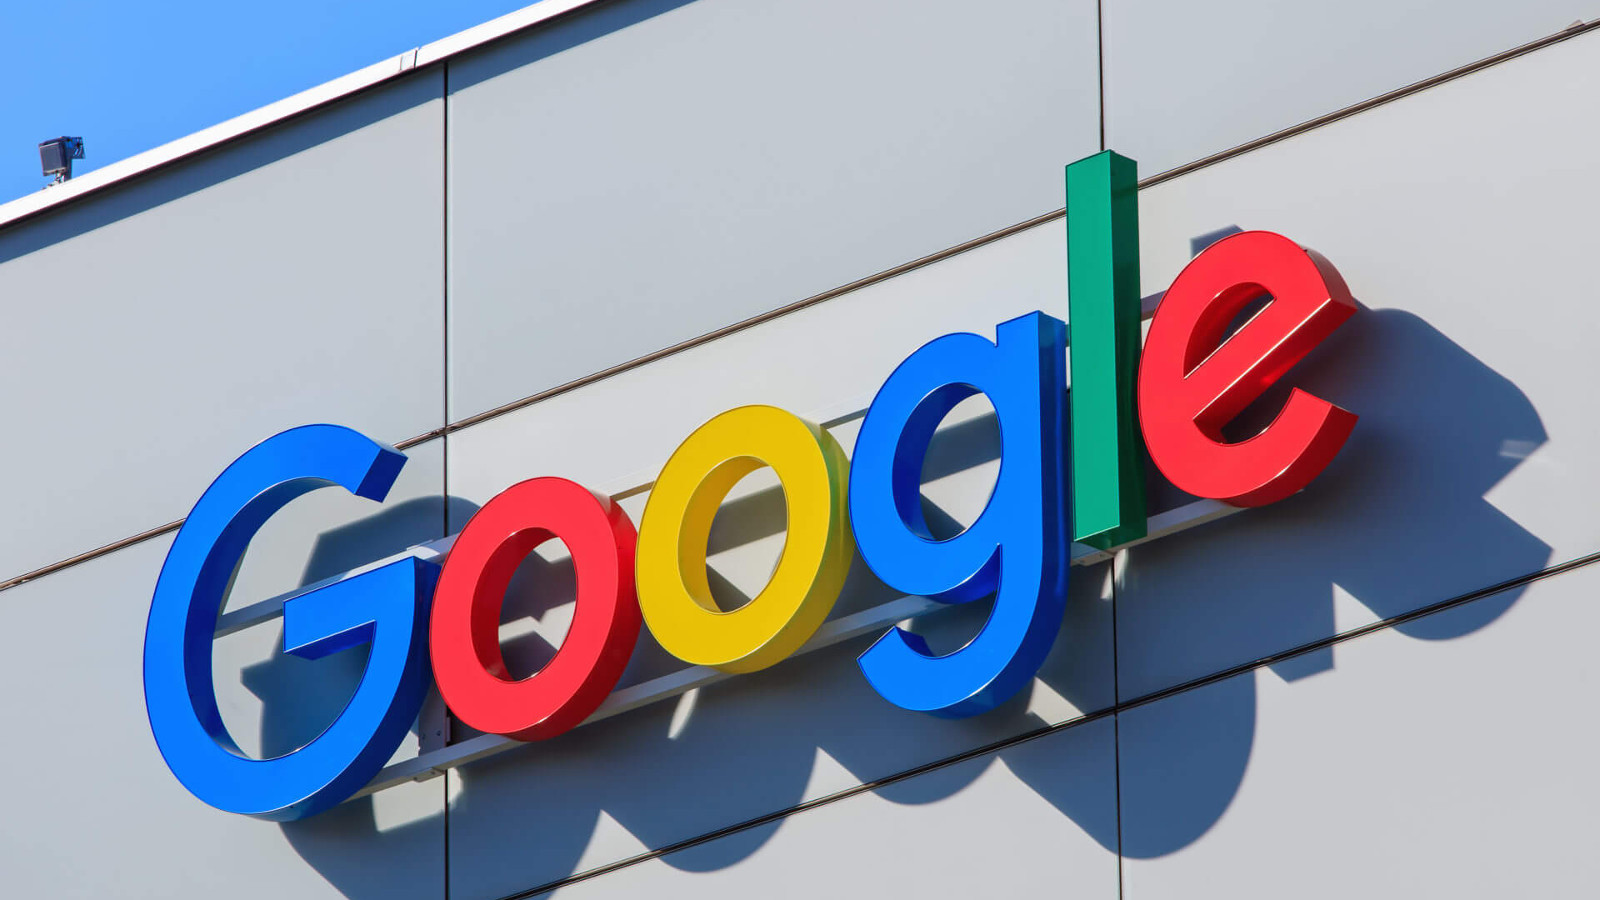
\includegraphics[height=\paperheight]{images/google-building-logo-shutterstock.jpg}}
    \begin{frame}
        \begin{titlebox}
            \centering
            {They're called Google}
        \end{titlebox}
    \end{frame}
    }

    {%
    \usebackgroundtemplate{\tikz\node[opacity=0.2,inner sep=0] {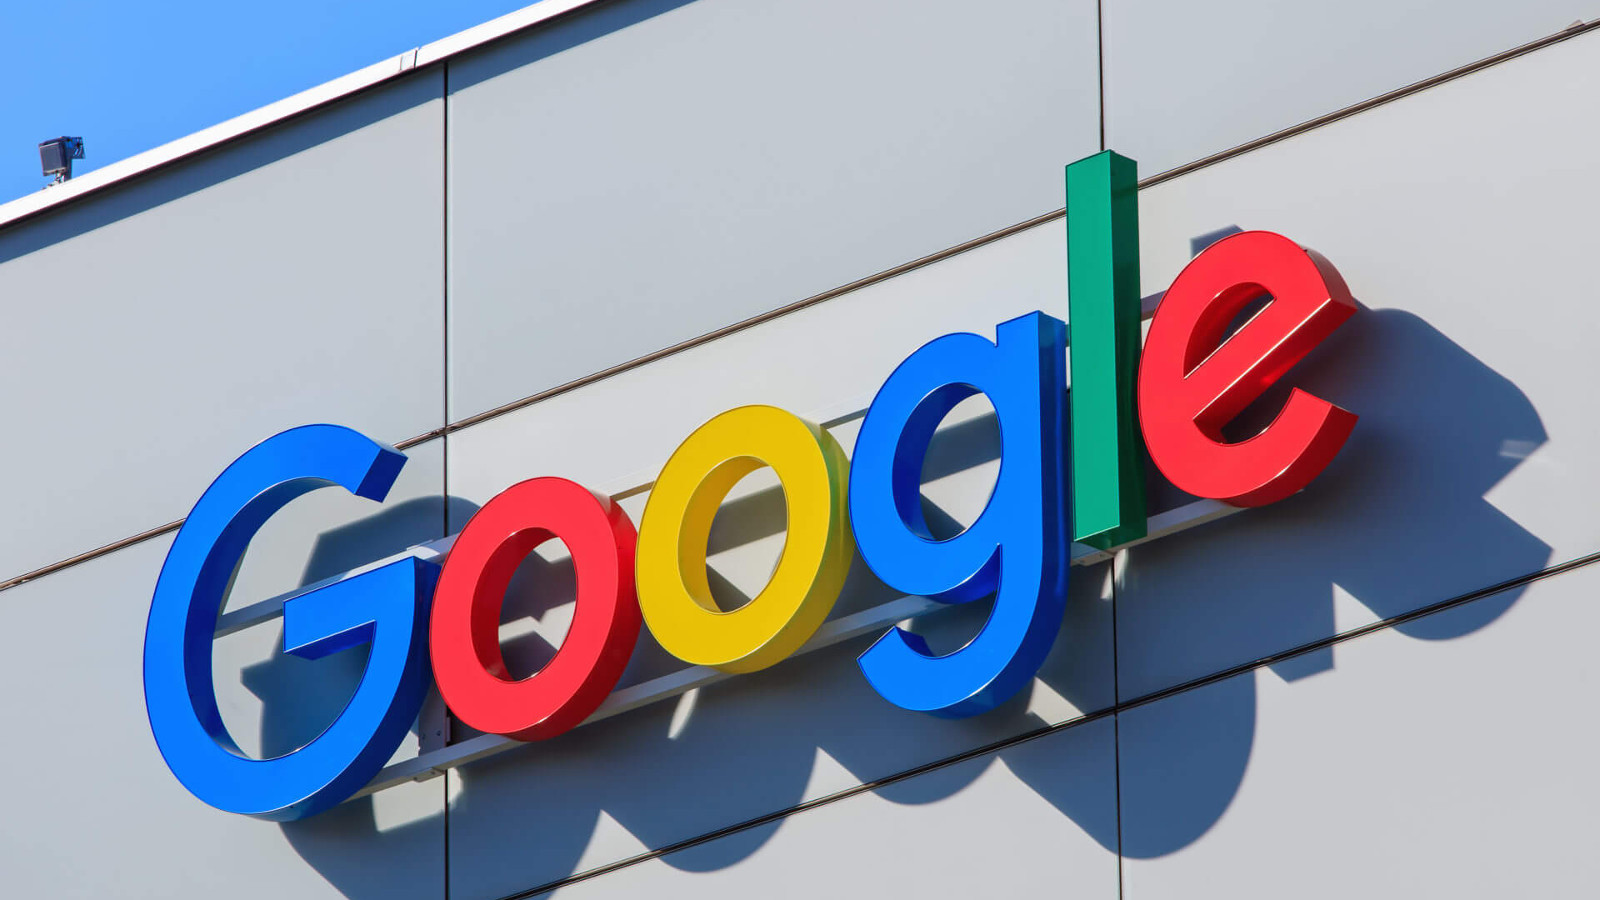
\includegraphics[height=\paperheight]{images/google-building-logo-shutterstock.jpg}};}
    \begin{frame}{Humble Beginnings}
        \begin{itemize}
            \item Founded in 1998, Google offers a search engine which allows
                users to find content on the (growing) World Wide Web
            \item Unfortunately, there's not really a lot of money to be made
                in this market at this time
            \item Google was earning income by selling search services to
                partners and providing ad services, but losing the race against
                her competitors
        \end{itemize}
    \end{frame}
    }

    {%
    \usebackgroundtemplate{\tikz\node[opacity=0.2,inner sep=0] {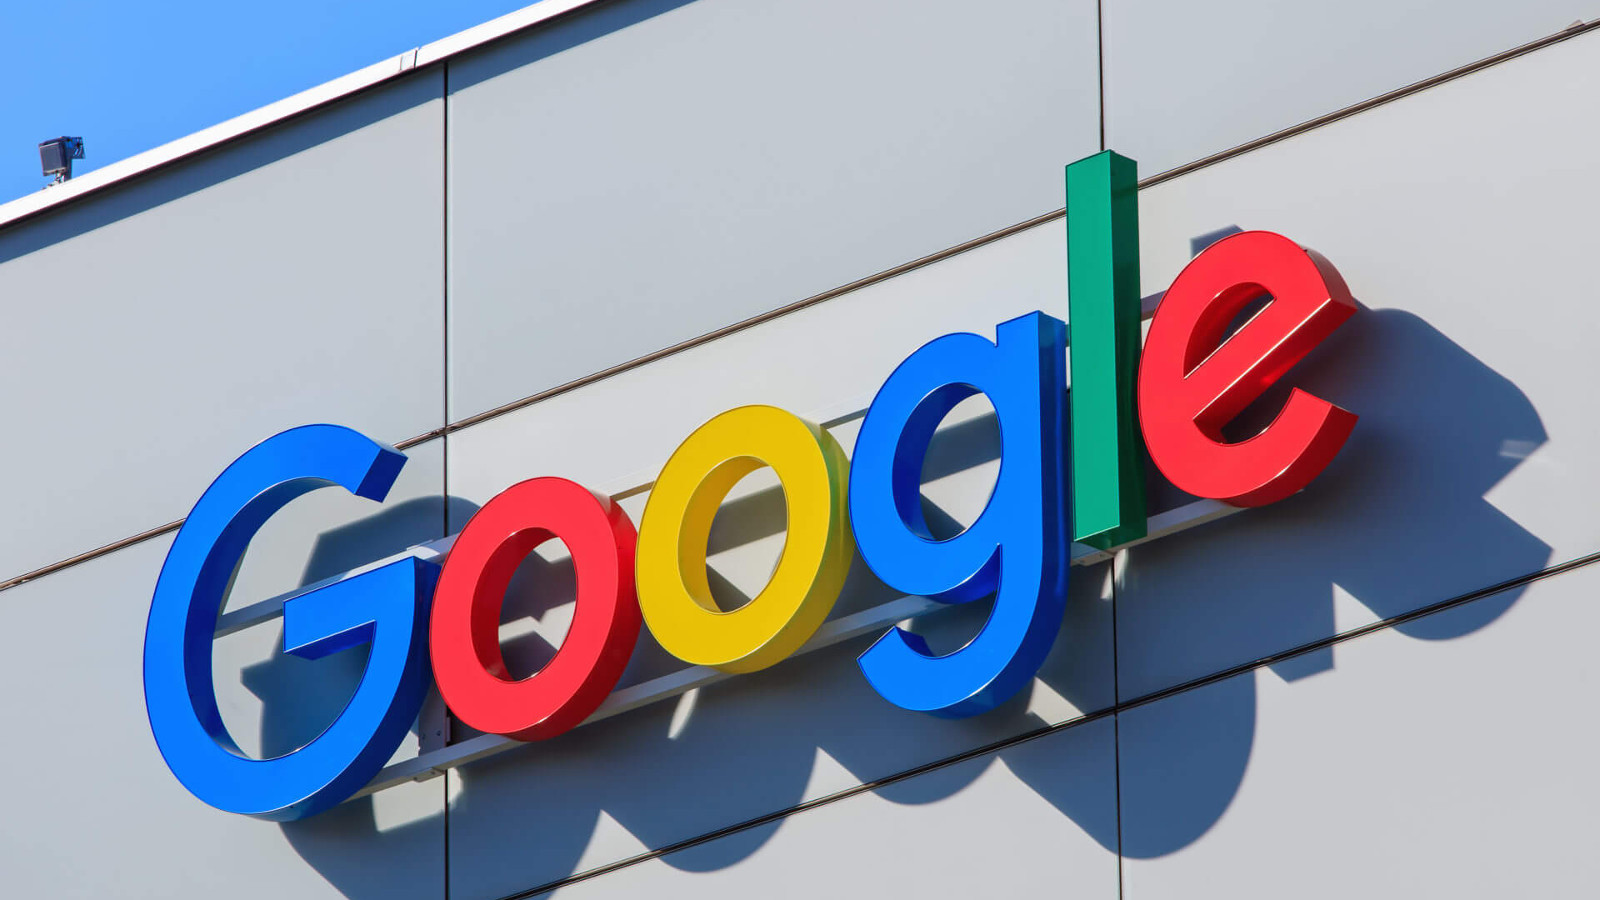
\includegraphics[height=\paperheight]{images/google-building-logo-shutterstock.jpg}};}
    \begin{frame}{Data Exhaust}
        \begin{itemize}
            \item Each search query produces a wake of collateral data, at this
                point in time mostly ignored
            \pause{}
            \item Once considered \alert{data exhaust}, this collateral data
                can be turned into a broad sensor of human behaviour:
                \alert{behavioural surplus}
            \pause{}
            \item A balance of power was maintained over the following years,
                with Google feeding user behaviour back into the search
                algorithm to improve results
        \end{itemize}
        \note[item]{Investment cycle benefits the user}
    \end{frame}
    }

    {%
    \usebackgroundtemplate{\tikz\node[opacity=0.2,inner sep=0] {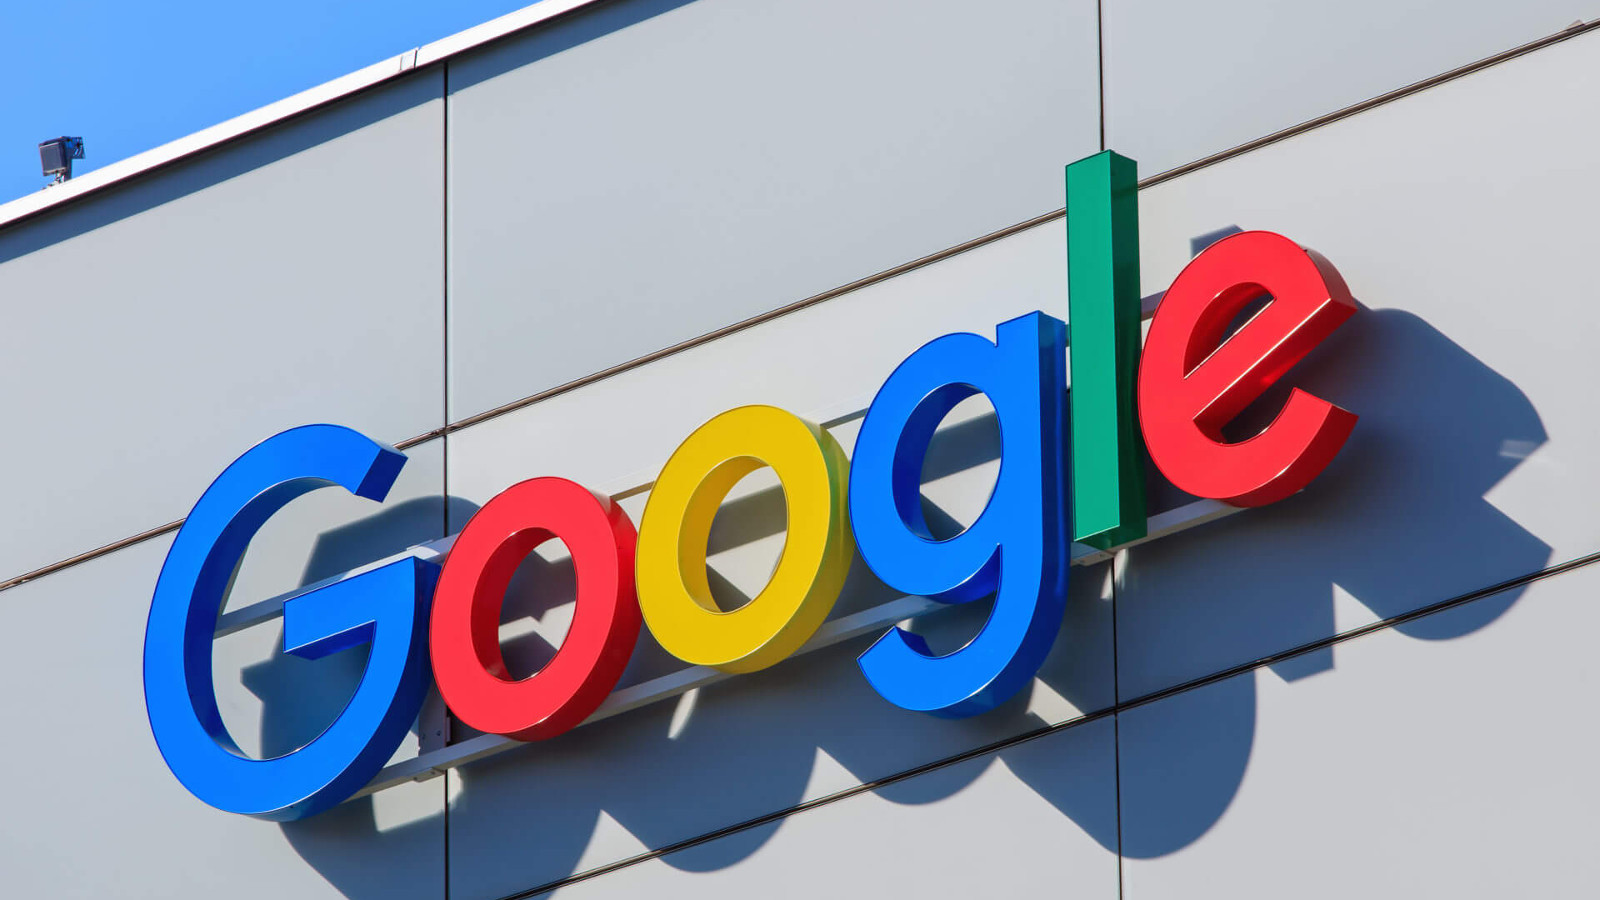
\includegraphics[height=\paperheight]{images/google-building-logo-shutterstock.jpg}};}
    \begin{frame}{Behavioural Surplus}
        \begin{itemize}
            \item In 2002, Google decides to start utilising it's substantial
                source of behavioural surplus for \alert{advertising}
            \item Ads must be relevant and targeted to the user, which is done
                by putting the behavioural surplus to work
            \pause{}
            \item All the instruments needed to individually track users online
                are created and put in place
            \item Google is no longer in the search business, but predicting
                what a user is going to do. In essence, it is selling
                \alert{prediction products}
        \end{itemize}
        \note[item]{Investment cycle no longer exclusively benefits the user}
        \note[item]{You are not the product, but your behaviour is}
    \end{frame}
    }

    {%
    \usebackgroundtemplate{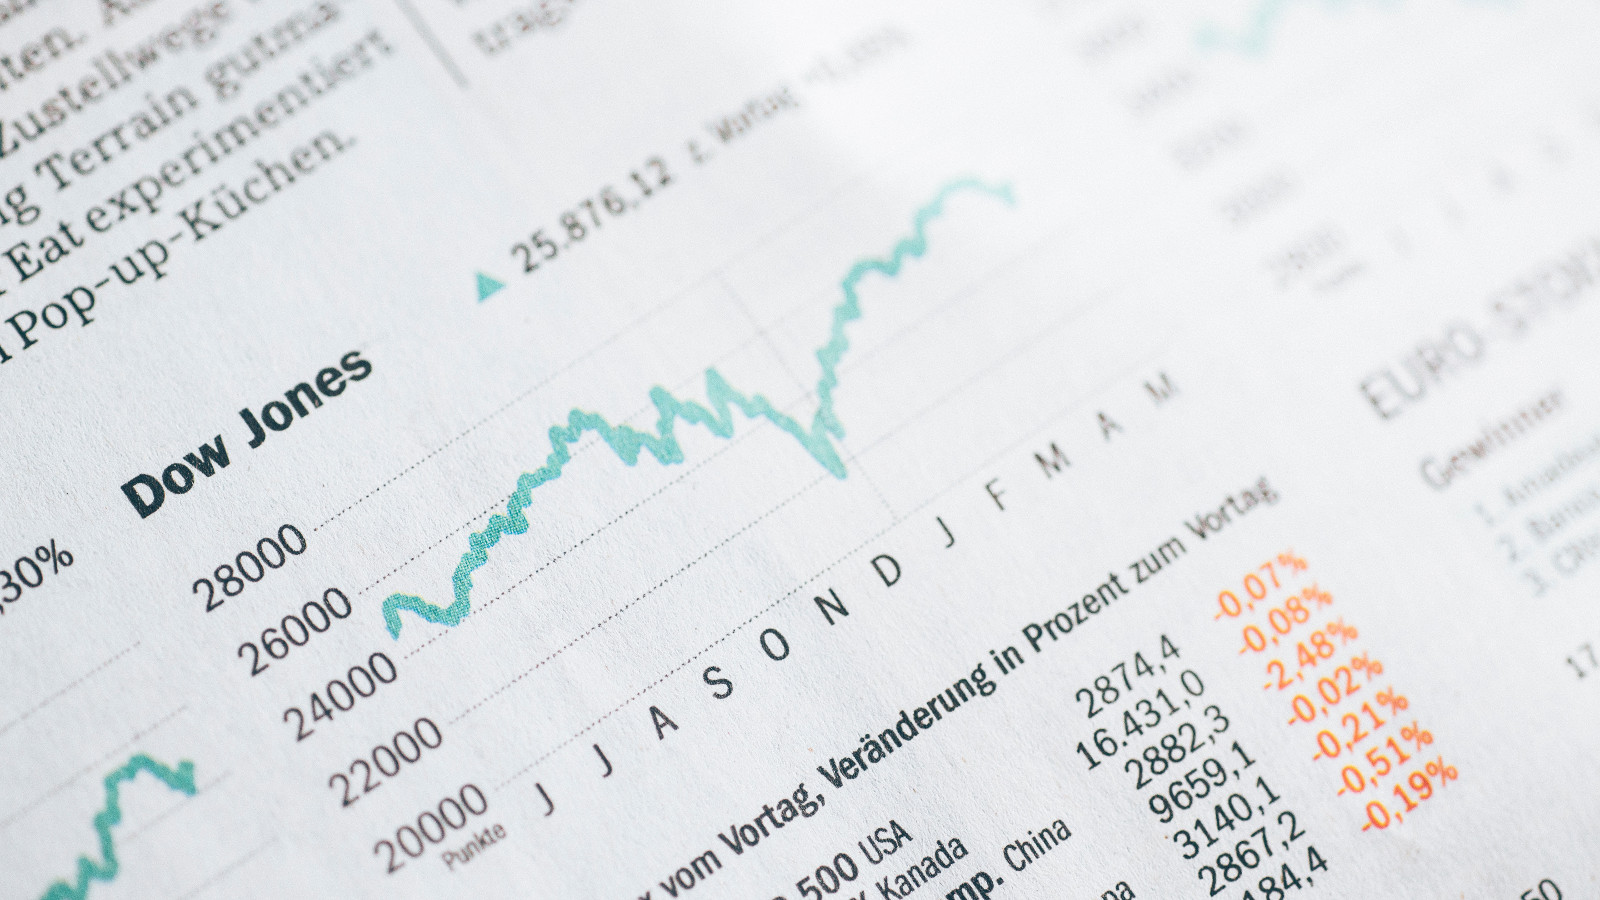
\includegraphics[height=\paperheight]{images/markus-spiske-unsplash.jpg}}
    \begin{frame}
        \begin{titlebox}
            \centering
            {Surveillance Capitalism}
        \end{titlebox}
        \note[item]{A new economic model is created, based on tracking and
            targeting users}
        \note[item]{Surveillance capitalists include Google, Facebook, Amazon,
            Apple \& Microsoft}
    \end{frame}
    }

    \section{Extraction \& Prediction Imperative}%
    \label{sec:extraction_prediction_imperative}

    {%
    \usebackgroundtemplate{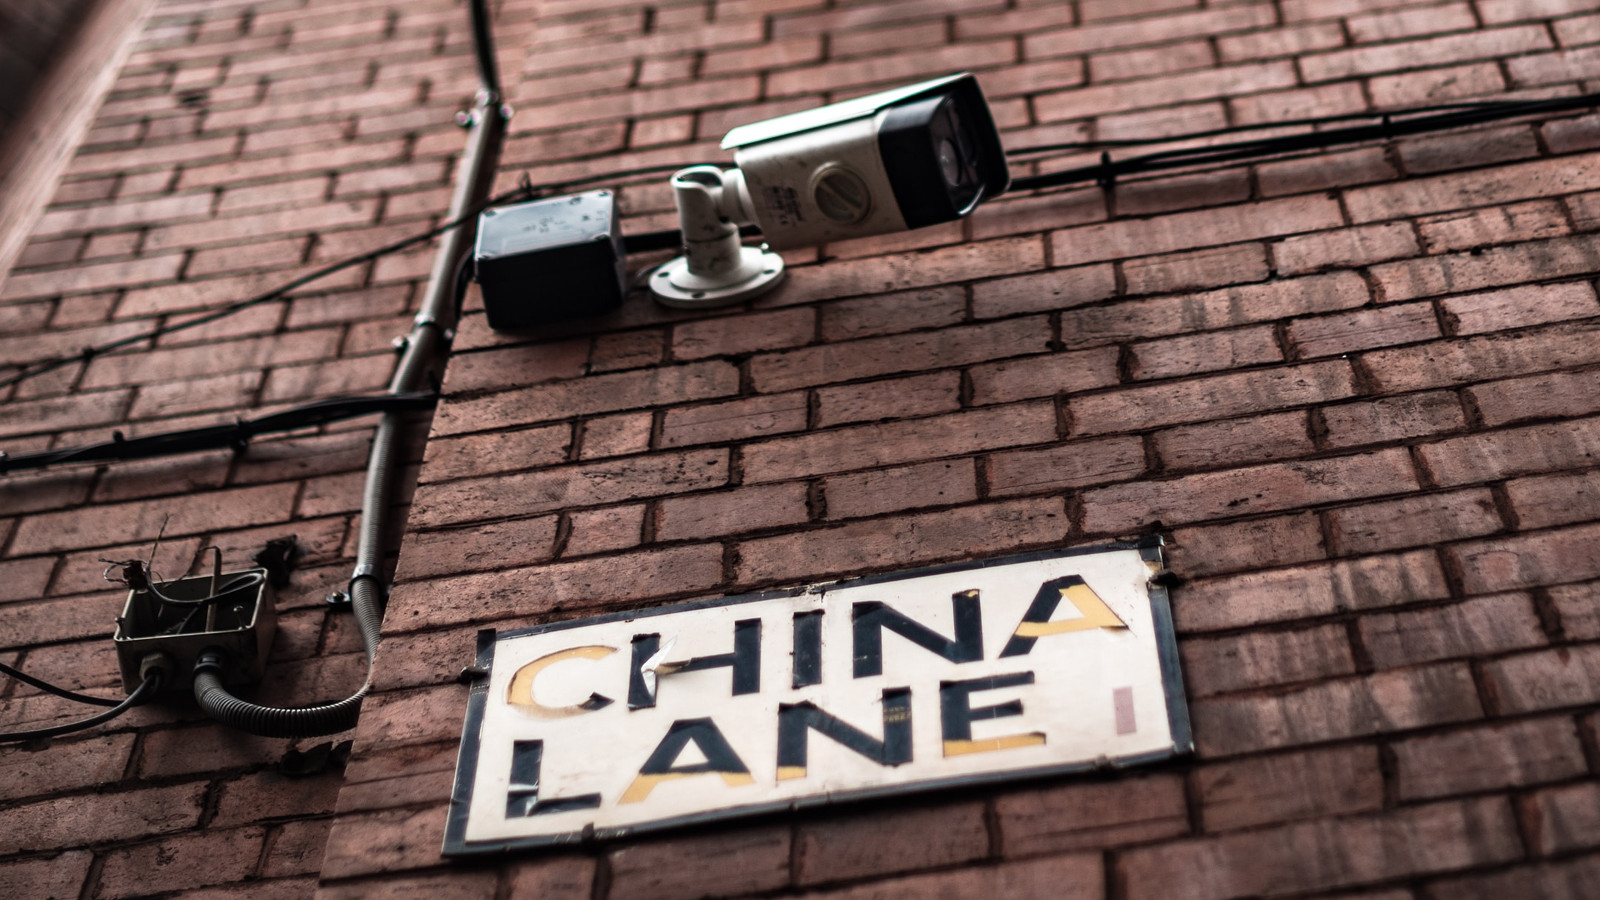
\includegraphics[height=\paperheight]{images/valentin-petkov-unsplash.jpg}}
    \begin{frame}
        \begin{titlebox}
            \centering
            {\emph{Imperative: having power to restrain, control, and direct}}
        \end{titlebox}
    \end{frame}
    }

    {%
    \usebackgroundtemplate{\tikz\node[opacity=0.2,inner sep=0] {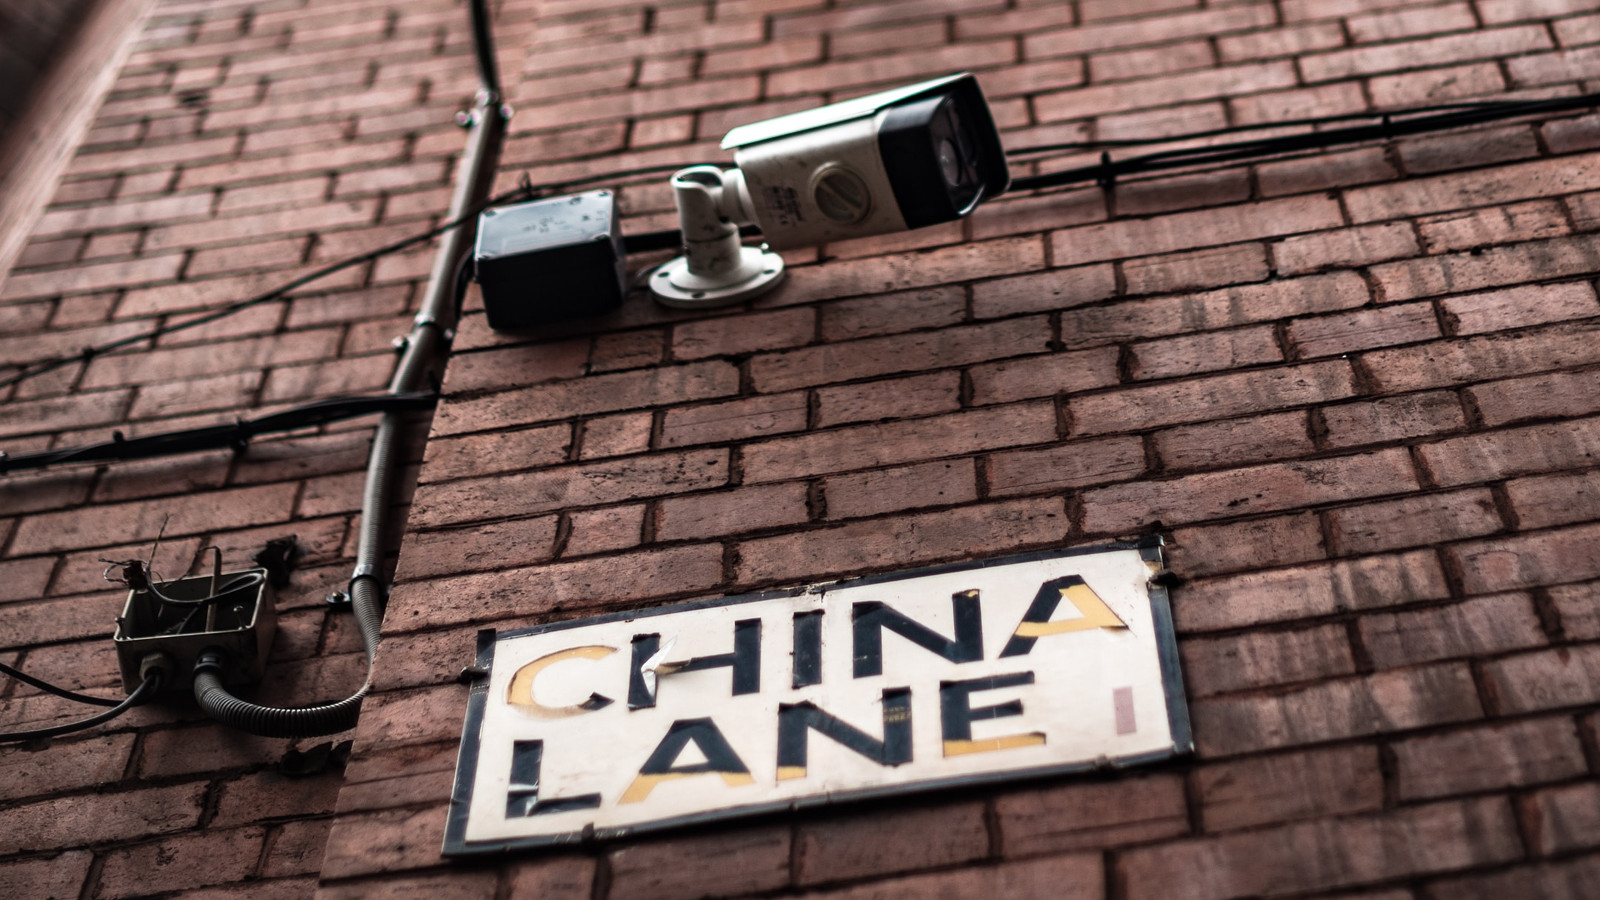
\includegraphics[height=\paperheight]{images/valentin-petkov-unsplash.jpg}};}
    \begin{frame}{Economy of Scale}
        \begin{itemize}
            \item As more behavioural surplus becomes available, the accuracy
                of predictions goes up
            \item As the accuracy of predictions go up, a higher price can be
                asked for \alert{prediction products}
            \pause{}
            \item As such, surveillance capitalists have an economic incentive
                to gather more and more behavioural surplus
            \item This behaviour is categorised as the \alert{extraction
                imperative}, creating an economy of scale
        \end{itemize}
        \note[item]{Tracking, capturing, analysing \& predicting}
    \end{frame}
    }

    {%
    \usebackgroundtemplate{\tikz\node[opacity=0.2,inner sep=0] {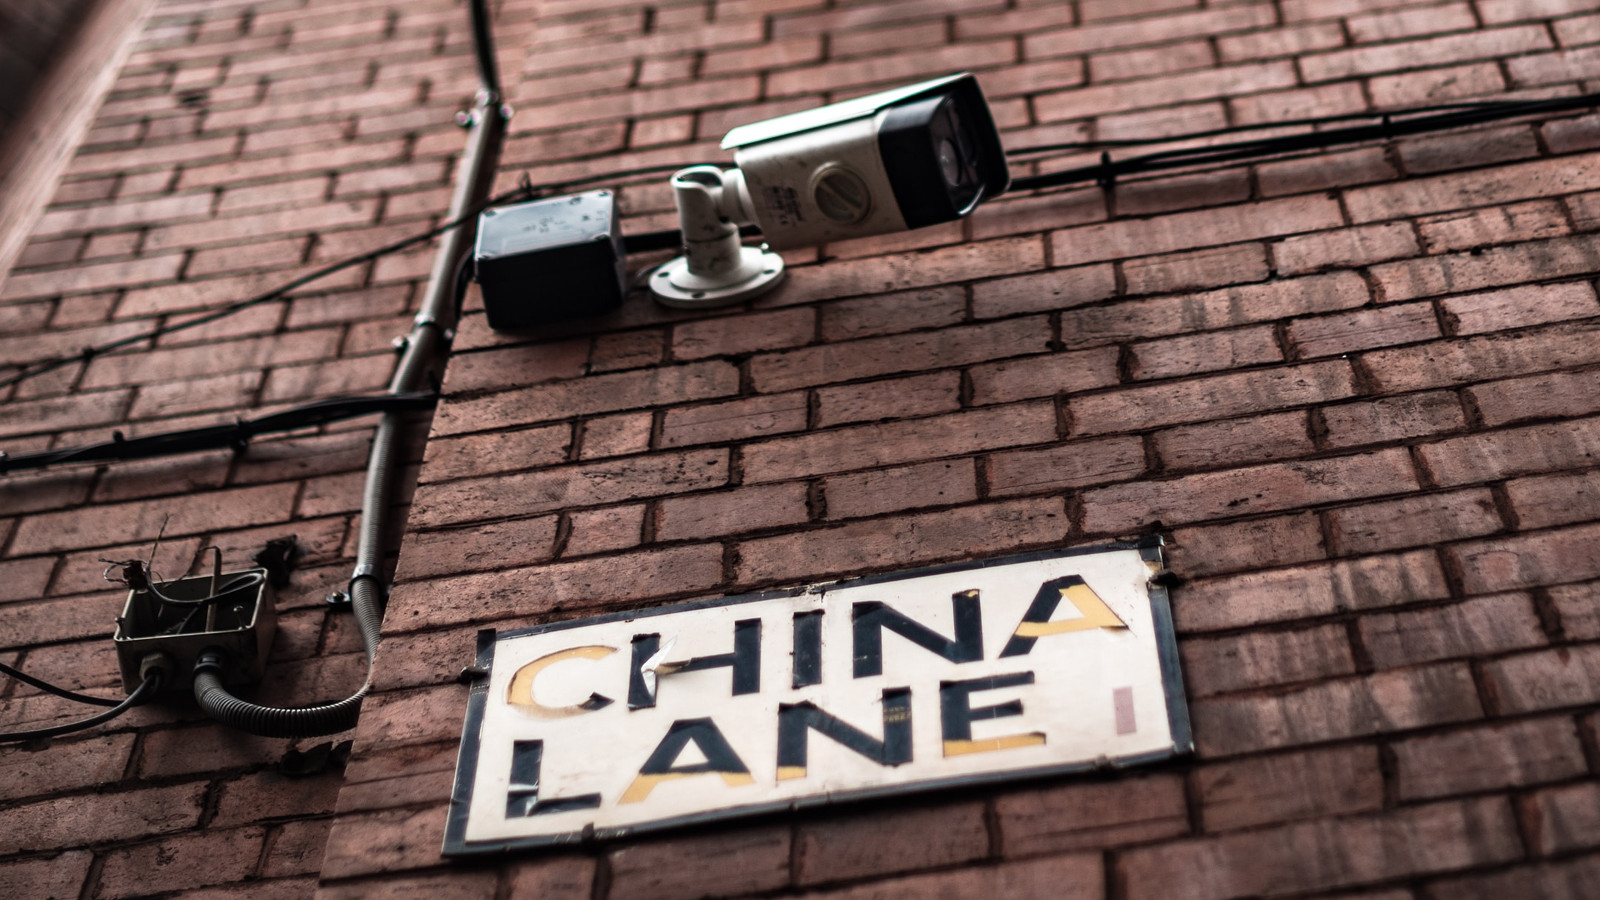
\includegraphics[height=\paperheight]{images/valentin-petkov-unsplash.jpg}};}
    \begin{frame}{If the Service is Free, You are the Product}
        \begin{itemize}
            \item By offering services for free, surveillance capitalists
                collect behavioural surplus
            \item Not wanting your data collected means not using the service
                (opt-out)
            \item Most people will still use the service, despite overwhelming
                abuse
            \pause{}
            \item Strictly speaking, you are not the product, but rather your
                behaviour is
        \end{itemize}
    \end{frame}
    }

    {%
    \usebackgroundtemplate{\tikz\node[opacity=0.3,inner sep=0] {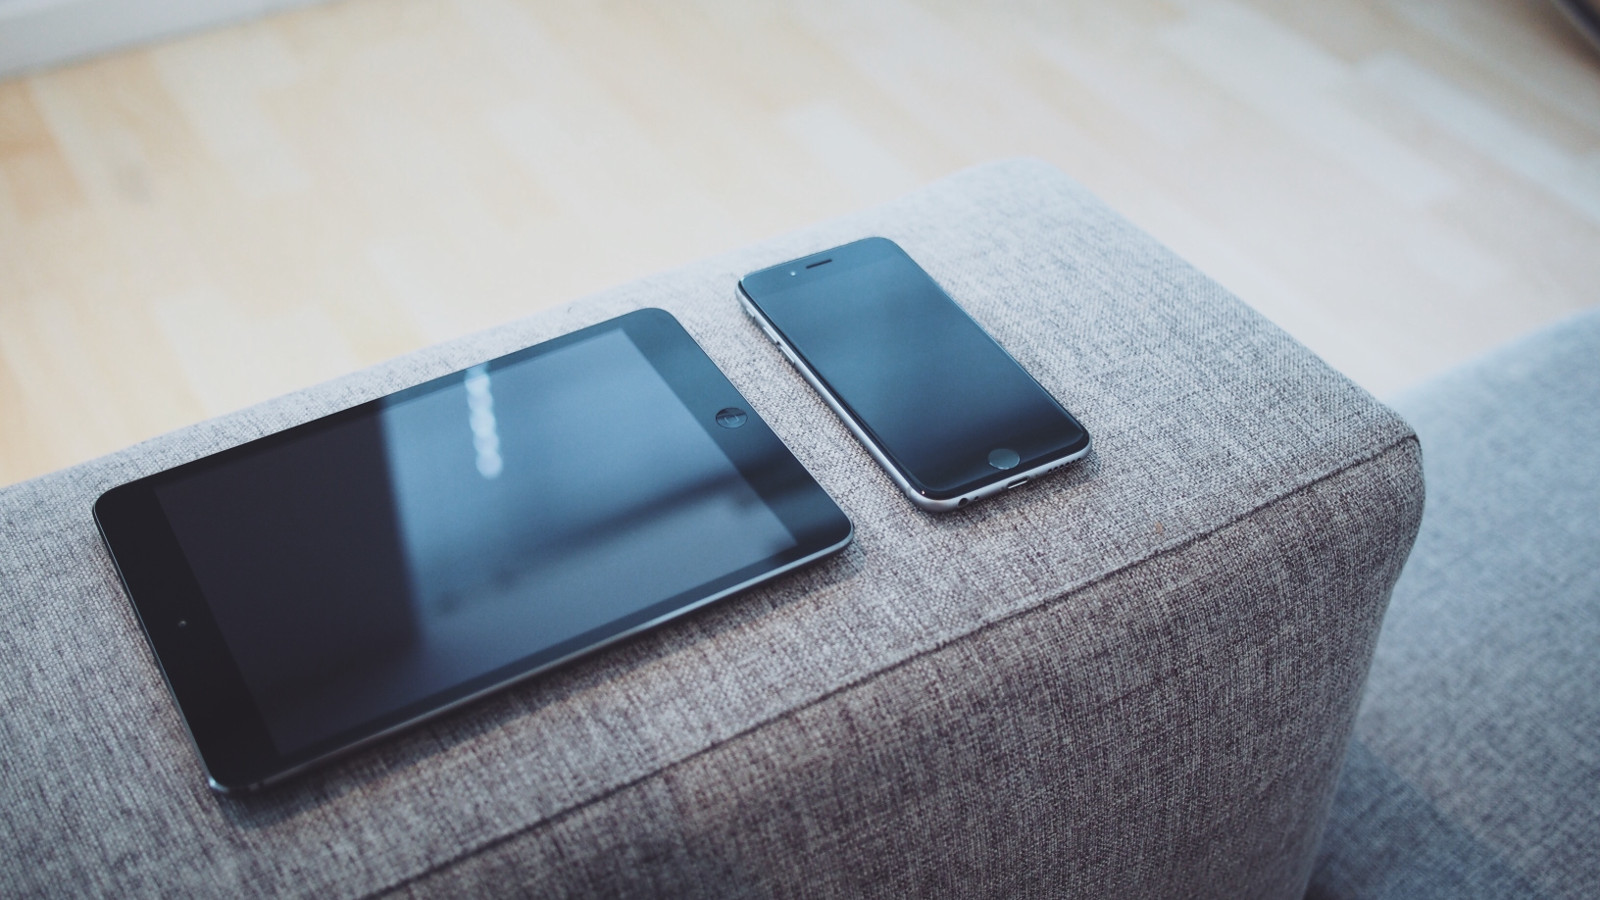
\includegraphics[height=\paperheight]{images/oliur-unsplash.jpg}};}
    \begin{frame}{Economy of Scope}
        \begin{itemize}
            \item With an ever growing hunger for more behavioural surplus,
                surveillance capitalism expands from the online world into the
                real world
            \pause{}
            \item One of the most basic and powerful aspects is location data
            \item Where are you? Where have you been? And where are you going?
            \pause{}
            \item Not only limited to personalised devices, but using sensors
                all around us (Internet of Things)
            \item This behaviour is categorised as the \alert{prediction
                imperative}, creating an economy of scope
        \end{itemize}
    \end{frame}
    }

    {%
    \usebackgroundtemplate{
\includegraphics[height=\paperheight]{images/pokemon-go-anniversary.jpg}}
    \begin{frame}
        \begin{titlebox}
            \centering
            {Pokémon Go}
        \end{titlebox}
    \end{frame}
    }

    {%
    \usebackgroundtemplate{\tikz\node[opacity=0.2,inner sep=0] {
\includegraphics[height=\paperheight]{images/pokemon-go-anniversary.jpg}};}
    \begin{frame}{Pokémon Go}
        \begin{itemize}
            \item A surveillance capitalist's dream-come-true
            \item Fusing scale \& scope, yielding continuous sources of behavioural
                surplus
            \item Became a living laboratory of conditioning and herding users
                through gamification
        \end{itemize}
    \end{frame}
    }

    \section{Guaranteed Outcomes}%
    \label{sec:guaranteed_outcomes}

    {%
    \usebackgroundtemplate{\tikz\node[opacity=0.2,inner sep=0] {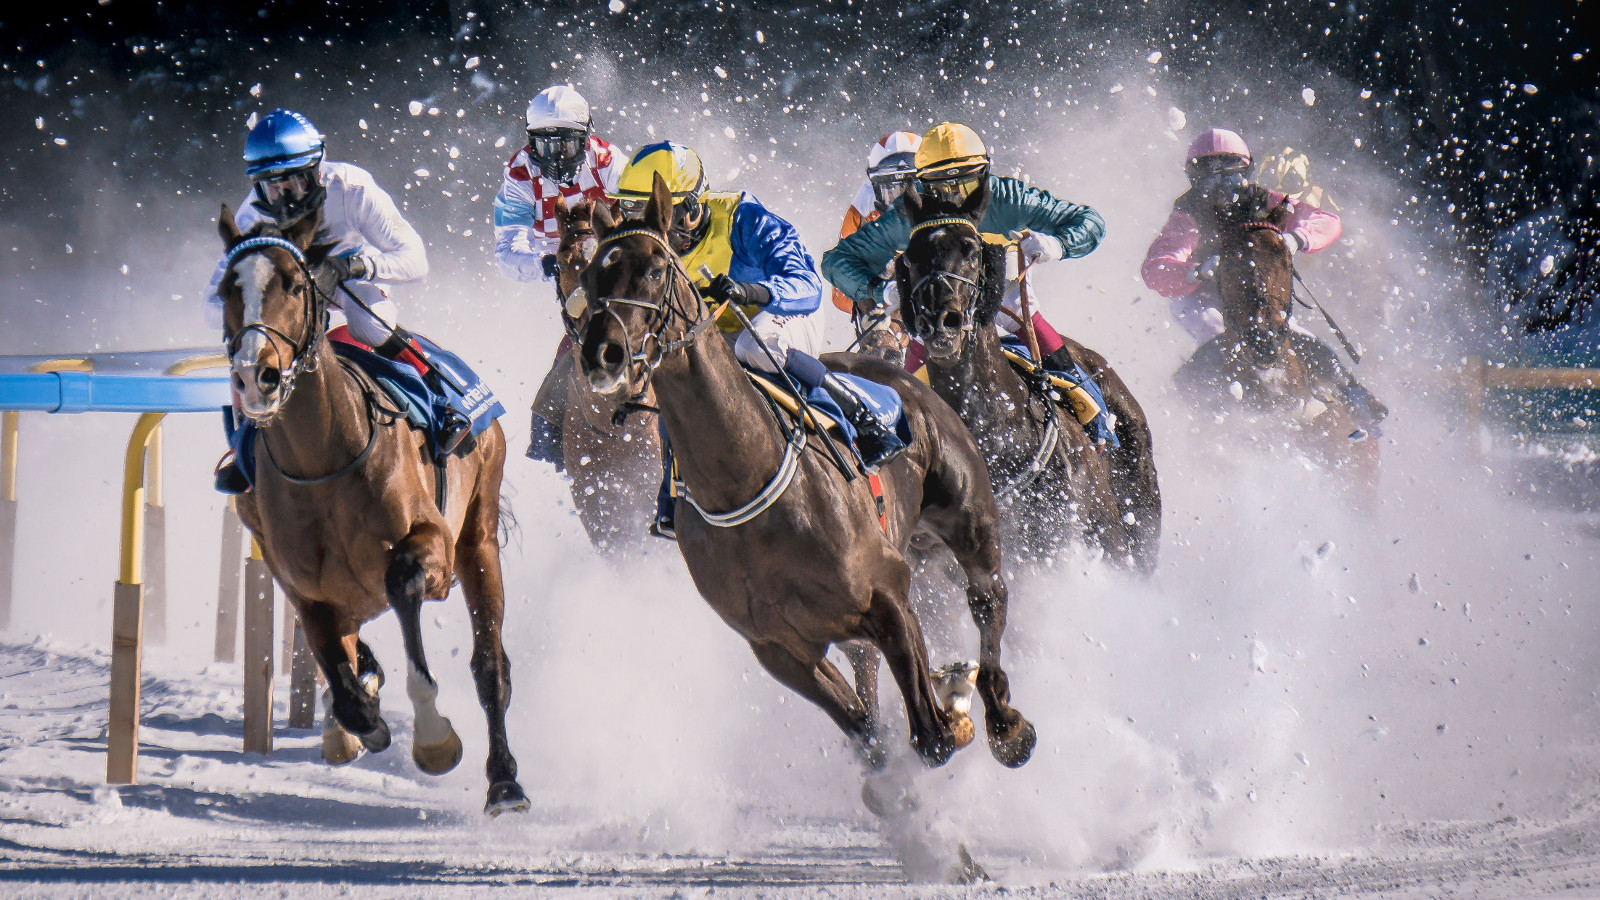
\includegraphics[height=\paperheight]{images/pietro-mattia-unsplash.jpg}};}
    \begin{frame}{Economy of Action}
        \begin{itemize}
            \item Surveillance capitalism requires ever more behavioural
                surplus to improve the accuracy of its prediction products
            \item But what if there's a way to move from passive collection of
                behavioural surplus to active behavioural modification?
            \pause{}
            \item Wouldn't it be nice to actively steer an individual to a
                specific guaranteed outcome?
            \pause{}
            \item In essence, can we actively influence the outcome to meet the
                prediction?
        \end{itemize}
    \end{frame}
    }

    {%
    \usebackgroundtemplate{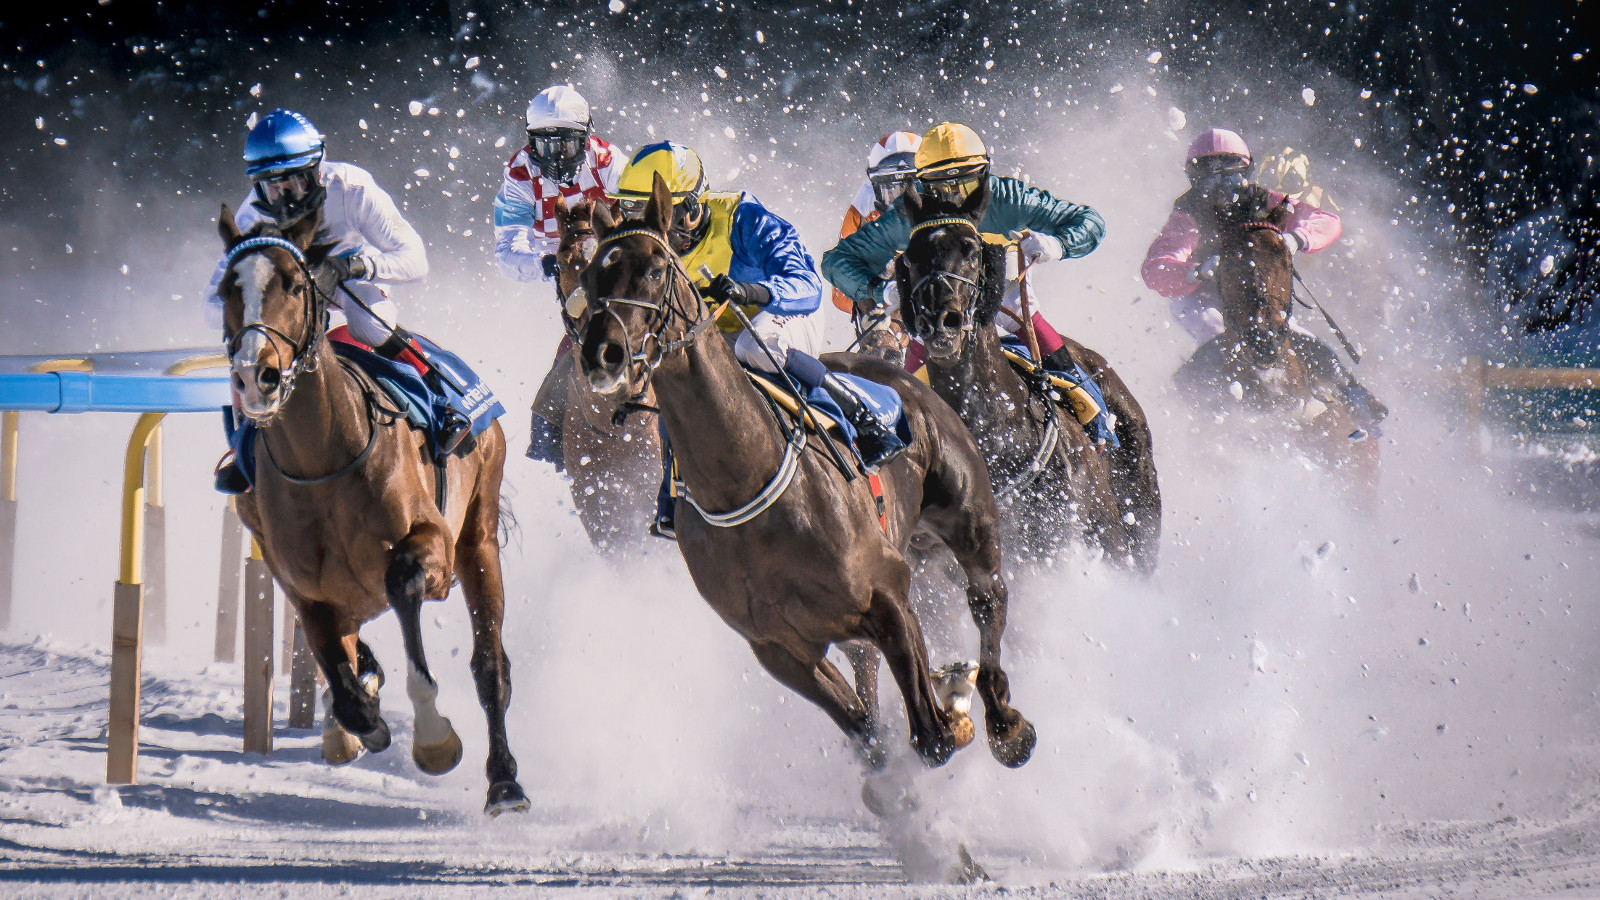
\includegraphics[height=\paperheight]{images/pietro-mattia-unsplash.jpg}}
    \begin{frame}
        \begin{titlebox}
            \centering
            {Economy of Action}
        \end{titlebox}
    \end{frame}
    }

    {%
    \usebackgroundtemplate{\tikz\node[opacity=0.2,inner sep=0] {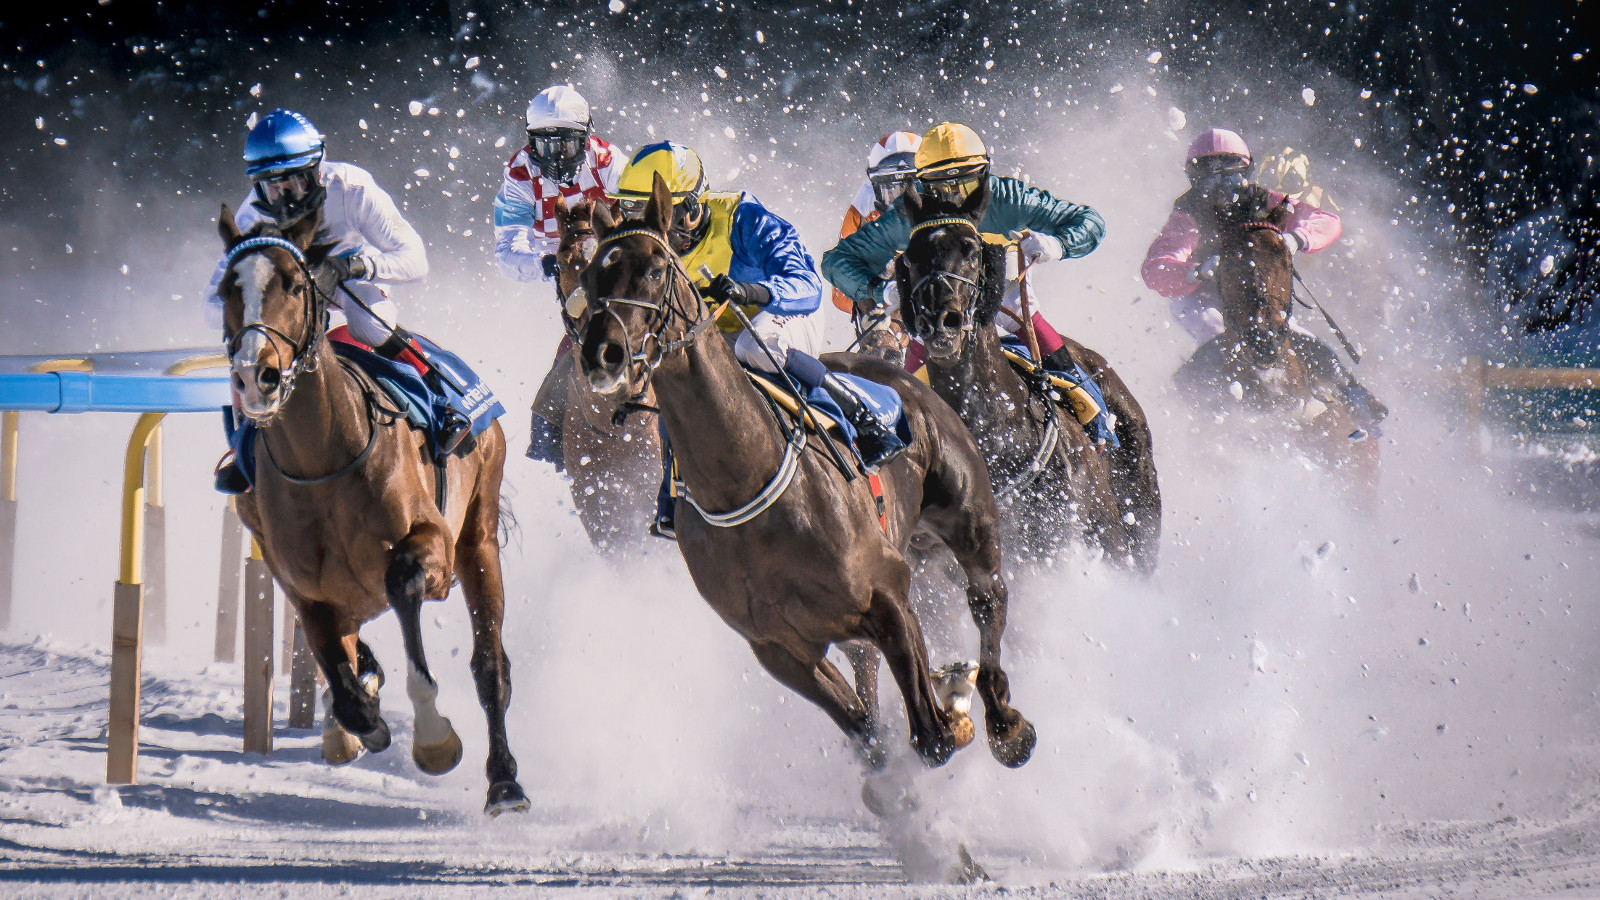
\includegraphics[height=\paperheight]{images/pietro-mattia-unsplash.jpg}};}
    \begin{frame}{Cambridge Analytica}
        \begin{itemize}
            \item Small UK-based consultancy firm, specialised in
                \alert{micro-behavioural targeting}
            \item Gathered large amounts of behavioural surplus, mostly on
                Facebook users through the use of questionnaires designed to
                gain access to user profiles
            \item Used this information to help influence the 2016 UK Brexit
                vote and US presidential election
            \pause{}
            \item Actively facilitated by Facebook, which makes money by
                selling prediction products
        \end{itemize}
    \end{frame}
    }

    {%
    \usebackgroundtemplate{\tikz\node[opacity=0.2,inner sep=0] {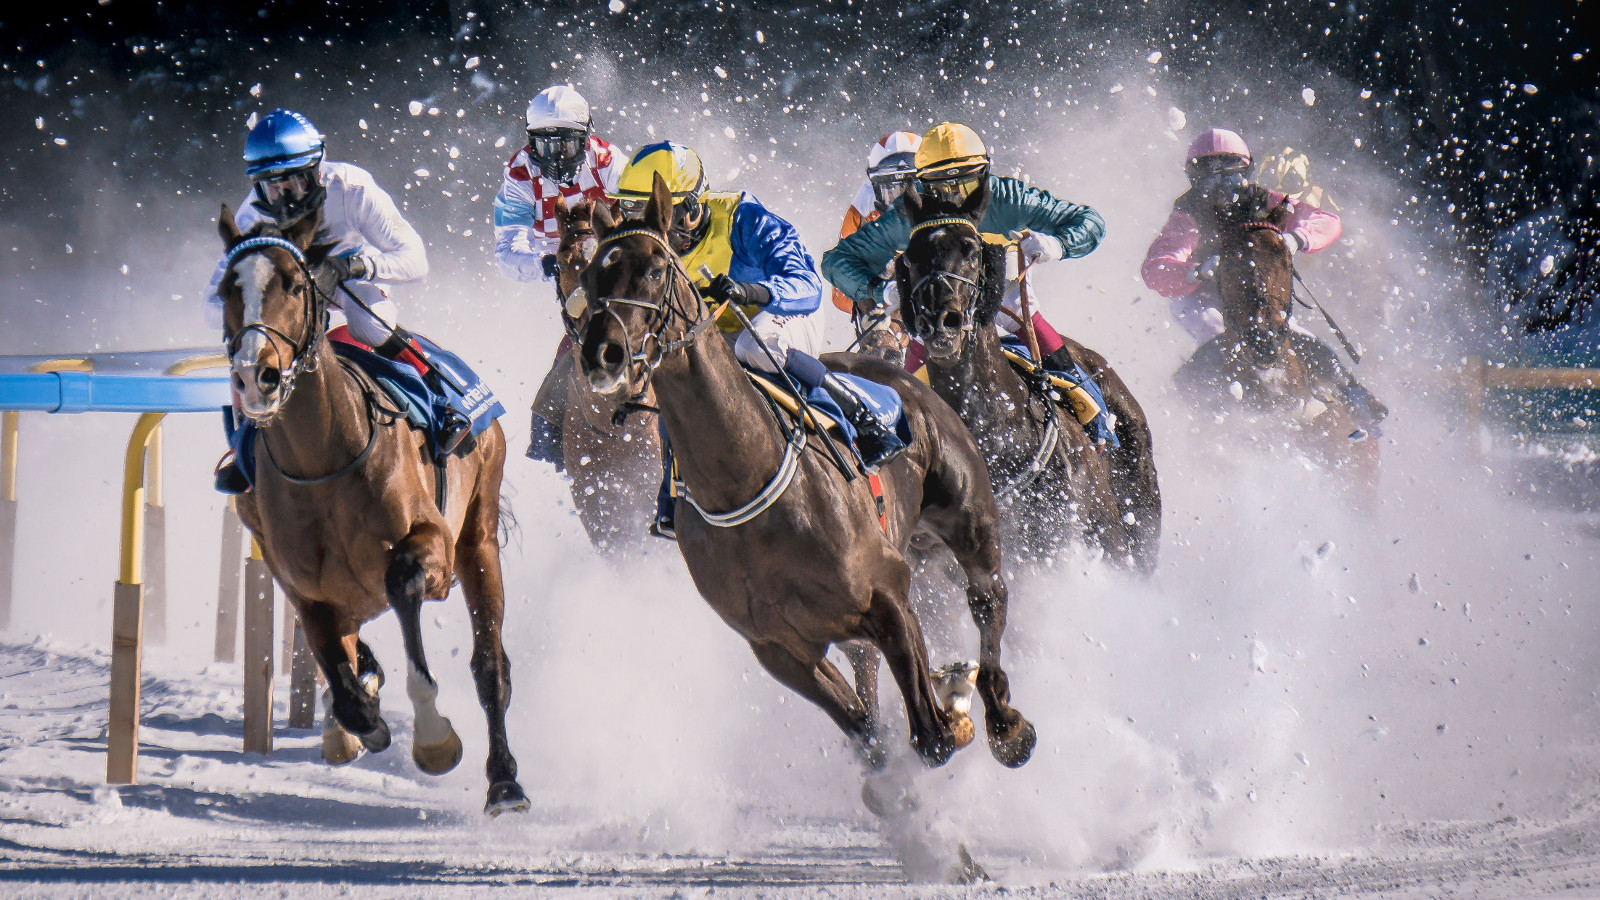
\includegraphics[height=\paperheight]{images/pietro-mattia-unsplash.jpg}};}
    \begin{frame}{Behavioural Modification}
        \begin{itemize}
            \item Tuning: shape the flow of behaviour to achieve maximum
                efficient influence. \alert{Nudges} a person to make a choice
                in a particular direction
            \pause{}
            \item Herding: controlling key elements in a person's immediate
                context, such as disabling a car when the driver is impaired
                (sense \& actuate)
            \pause{}
            \item Conditioning: defining a schedule of reinforcements, which
                includes rewards, recognition or praise
            \pause{}
            \item Be aware of the euphimism: \alert{personalisation}
        \end{itemize}
    \end{frame}
    }

    \section{Right to a Future Tense}%
    \label{sec:right_to_a_future_tense}

    {%
    \usebackgroundtemplate{\tikz\node[opacity=0.4,inner sep=0] {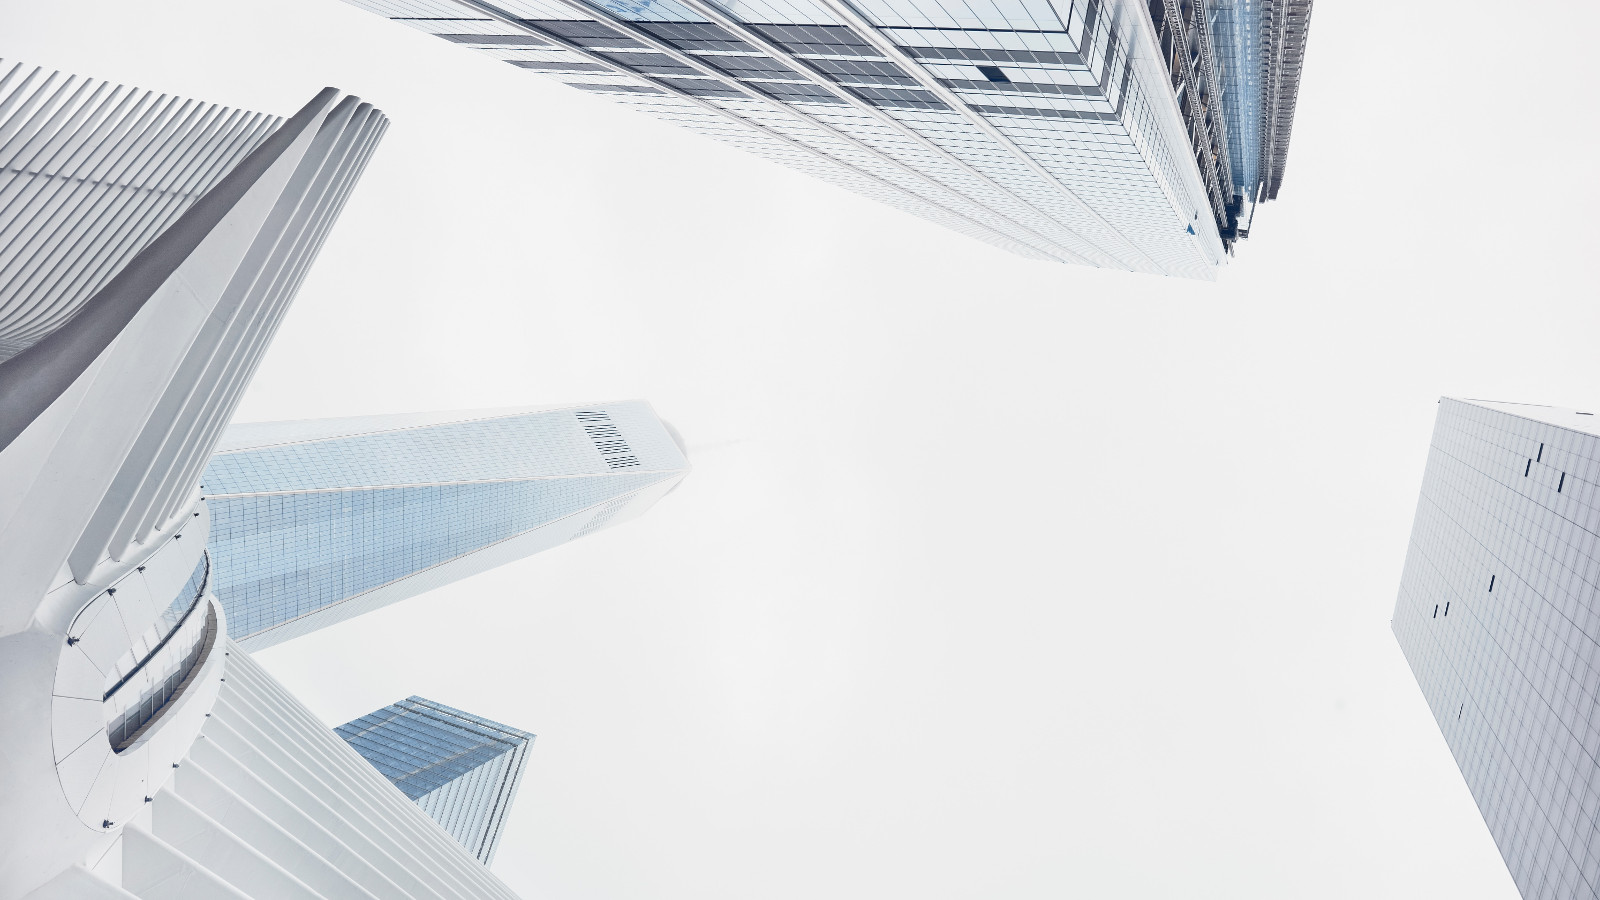
\includegraphics[height=\paperheight]{images/luca-bravo-unsplash.jpg}};}
    \begin{frame}{Right to a Future Tense}
        \begin{itemize}
            \item Everything you do is tracked, captured, analysed and sold to
                the highest bidder as part of a \alert{prediction product}
            \item You are being manipulated into a \alert{guaranteed outcome},
                while someone else profits
            \pause{}
            \item Are you angry yet?
        \end{itemize}
        \note[item]{You deserve not to be manipulated. You deserve the right to
            access information. You deserve to make your own choices and
            mistakes}
    \end{frame}
    }

    {%
    \usebackgroundtemplate{\tikz\node[opacity=0.4,inner sep=0] {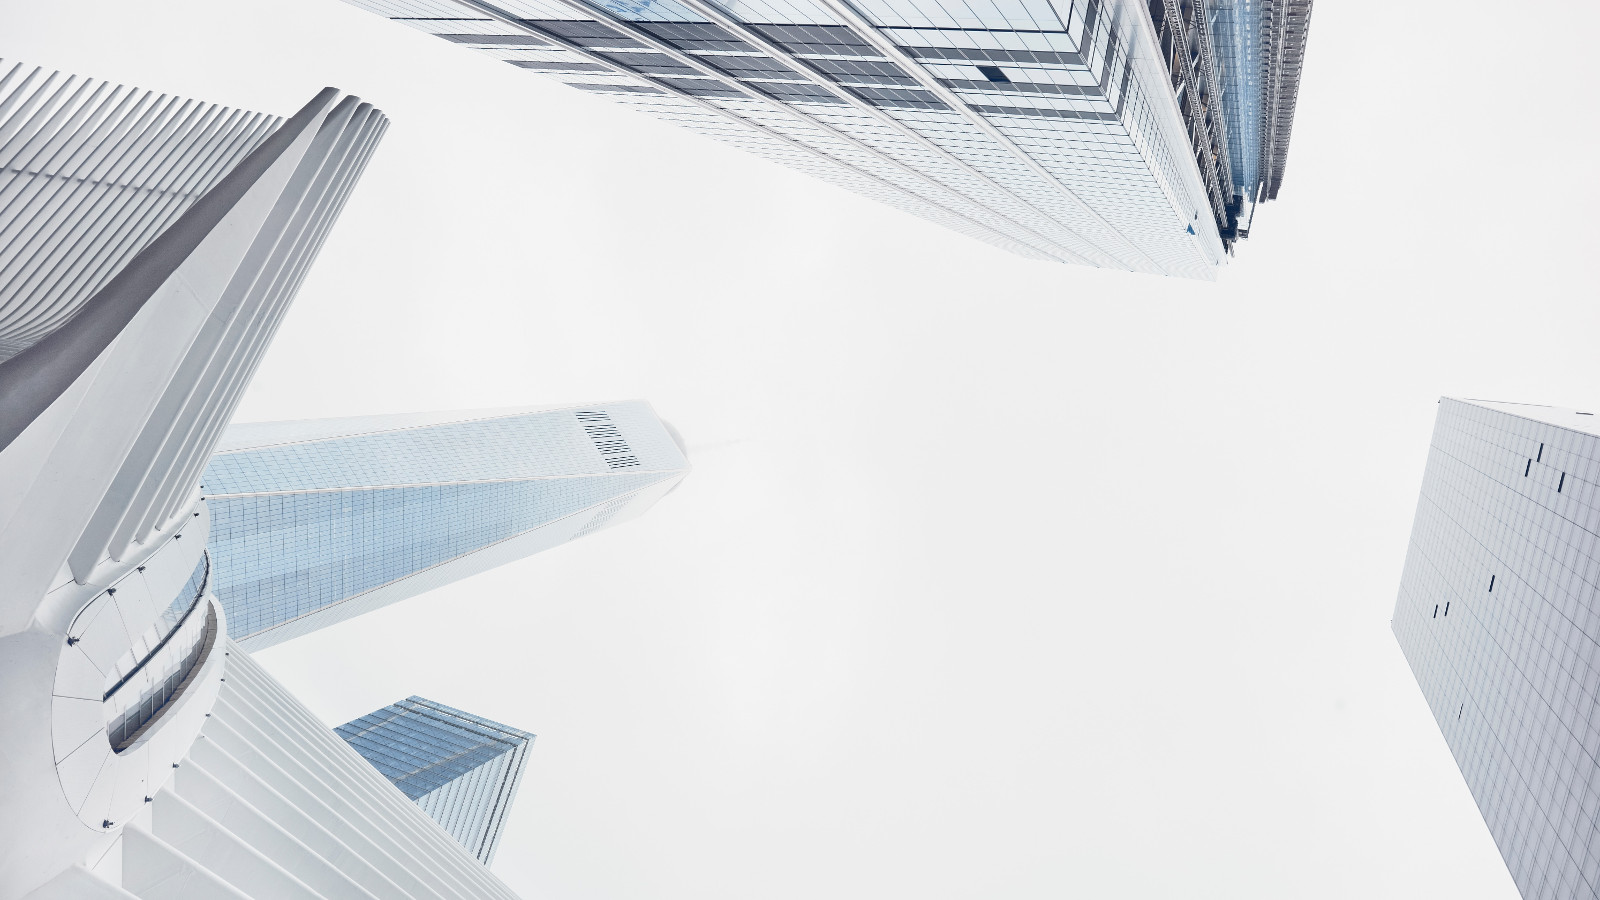
\includegraphics[height=\paperheight]{images/luca-bravo-unsplash.jpg}};}
    \begin{frame}{Right to a Future Tense}
        \begin{itemize}
            \item What happens when your government gets access to all this
                behavioural surplus?
            \pause{}
            \item What happens when your government fails to regulate the
                collection of behavioural surplus?
            \pause{}
            \item What happens when behavioural surplus is used to actively
                suppress your population?
            \pause{}
            \item Are you angry now?
        \end{itemize}
    \end{frame}
    }

    {%
    \usebackgroundtemplate{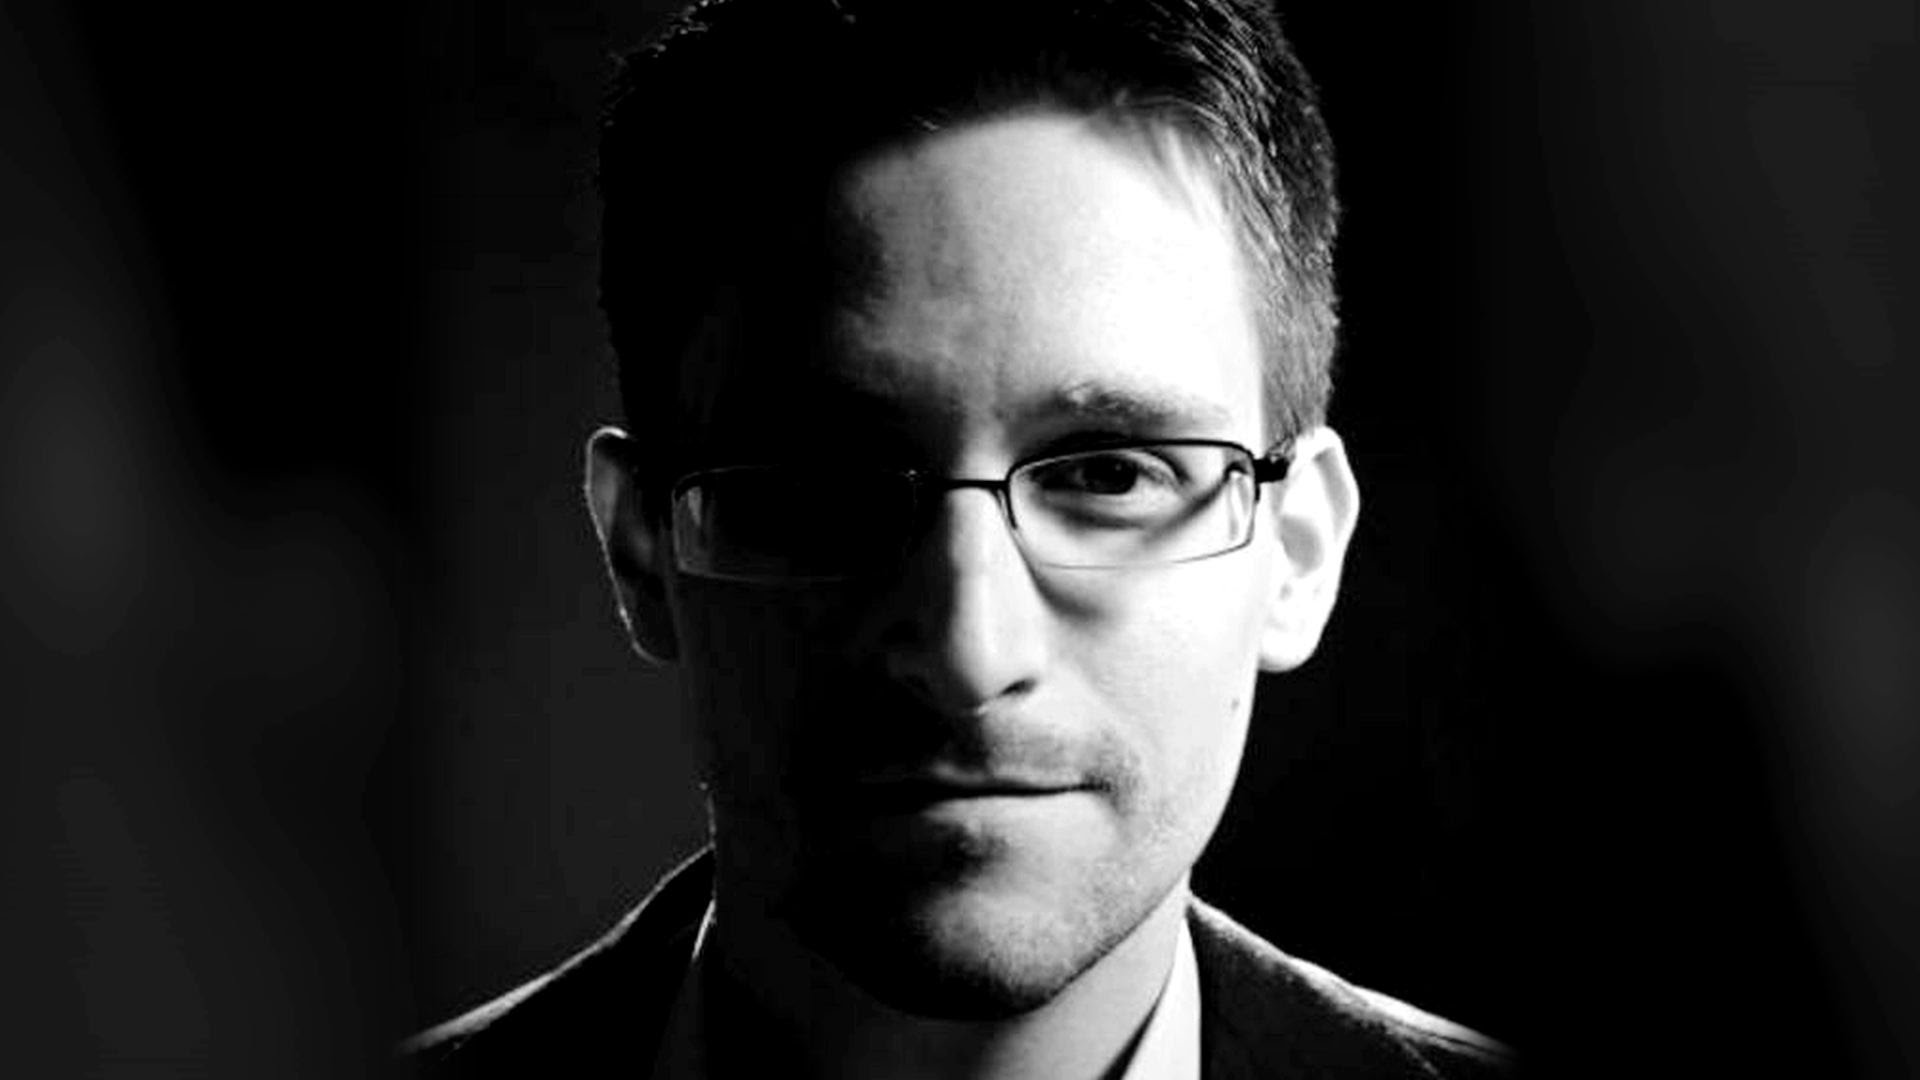
\includegraphics[height=\paperheight]{images/edward-snowden.jpg}}
    \begin{frame}
        \begin{titlebox}
            \centering
            {Encryption Works!}
        \end{titlebox}
    \end{frame}
    }

    \begin{frame}{License}
        Learn more \& get the source of this presentation from:
        \begin{center}\url{github.com/r1tger/crypto-party}\end{center}
        Licensed under \href{http://creativecommons.org/licenses/by-sa/4.0/}{Creative Commons Attribution-ShareAlike 4.0}.
        \begin{center}\ccbysa\end{center}
    \end{frame}

    \begin{frame}[standout]
        Questions?
    \end{frame}
\end{document}
